
As the charged Higgs Boson decays to a charm and an anti-strange quark, the
identification of charm jet is expected to increase the signal significance.
The charm tagging or c-tagging is recently developed in the CMS collaboration
~\cite{CMS-PAS-BTV-16-001} based on the CSV method for the analyses at 13 TeV 
data. This procedure is similar to that of b-tagging described in 
Section~\ref{s:bTag}. At the end, we have two charm discriminators: charm 
vs. b-jet (pfCCvsB) and charm vs. light jet (pfCCvsL). Distribution of these 
two discriminators is shown in Figure~\ref{fig:pfCCvsBL} for the \mujets and
\ejets channel. These are collectively used to tag a jet as a c-jet.
Three working points are provided by BTV POG for the charm tagging, as shown 
in Table (\ref{tab:cTagEff}) and Figure~\ref{fig:cTagger}.

At least one of the light jets from hadronic decay mode of \ttbar is required 
to pass one of the charm-jet working points. First, each WP was separately used
for c-tagging. However, the limits were not getting improved for medium and tight 
working points. Therefore the loose WP is finally used. Although the signal to
background ratio increases as one goes from loose to tight working point, 
the limits are not improved because the event yield also goes down. However,
it is found that, as described in Section (\ref{ss:mjj_cTagEx}), that if the 
events after KinFit selection are exclusively divided into the categories 
based on loose, medium, and the tight charm working points and the limit is 
computed by combining data cards from these three categories, as described in 
Section (\ref{ss:limit_cTagEx}), then the limit is improved.
\begin{table}
\caption{The efficiency of loose, medium, and tight c-tag working points for
    different quark-flavor of jets \cite{Sirunyan:2017ezt}. These efficiencies 
    are calculated from
\ttbar events with jet \pt $>$ 20 GeV.}
\label{tab:cTagEff}
\begin{center}
\begin{tabular}{cccccc}
\hline
\hline
WP & $\epsilon^c$ (\%) & $\epsilon^b$ (\%) & $\epsilon^{udsg}$ (\%) & pfCCvsL & pfCBvsB\\ \hline\hline
c-tagger L & 88 & 36 & 91 & $>$ -0.48 & $>$ -0.17 \\
c-tagger M & 40 & 17 & 19 & $>$ -0.1  & $>$  0.08 \\
c-tagger T & 19 & 20 & 1.2& $>$ 0.69  & $>$ -0.45 \\
\hline
\end{tabular}
\end{center}
\end{table}
%ctag eff figure
\begin{figure}
\centering
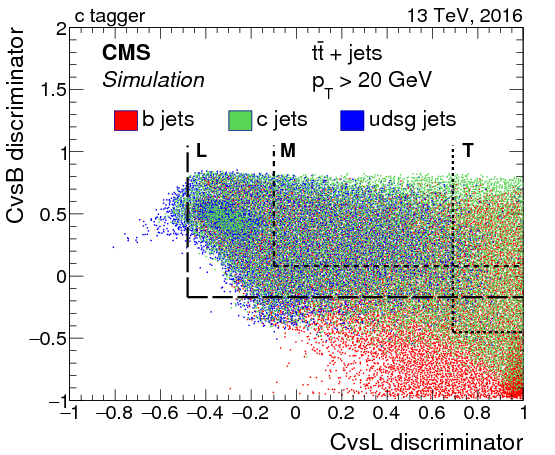
\includegraphics[width=0.6\linewidth]{Image/cTagger.png}
\caption{The 2D plot between charm-taggers. The region right to the vertical 
    and above to the horizontal line correspond to different charm working 
    points (WPs). Unlike the b-tag WPs, there is an overlap between the loose,
    medium, and tight c-tag WPs. This figure is taken from
~\cite{CMS-PAS-BTV-16-001}.}
\label{fig:cTagger}
\end{figure}

\begin{figure}
\centering
\subfigure[charm vs. b-jet discriminator ]{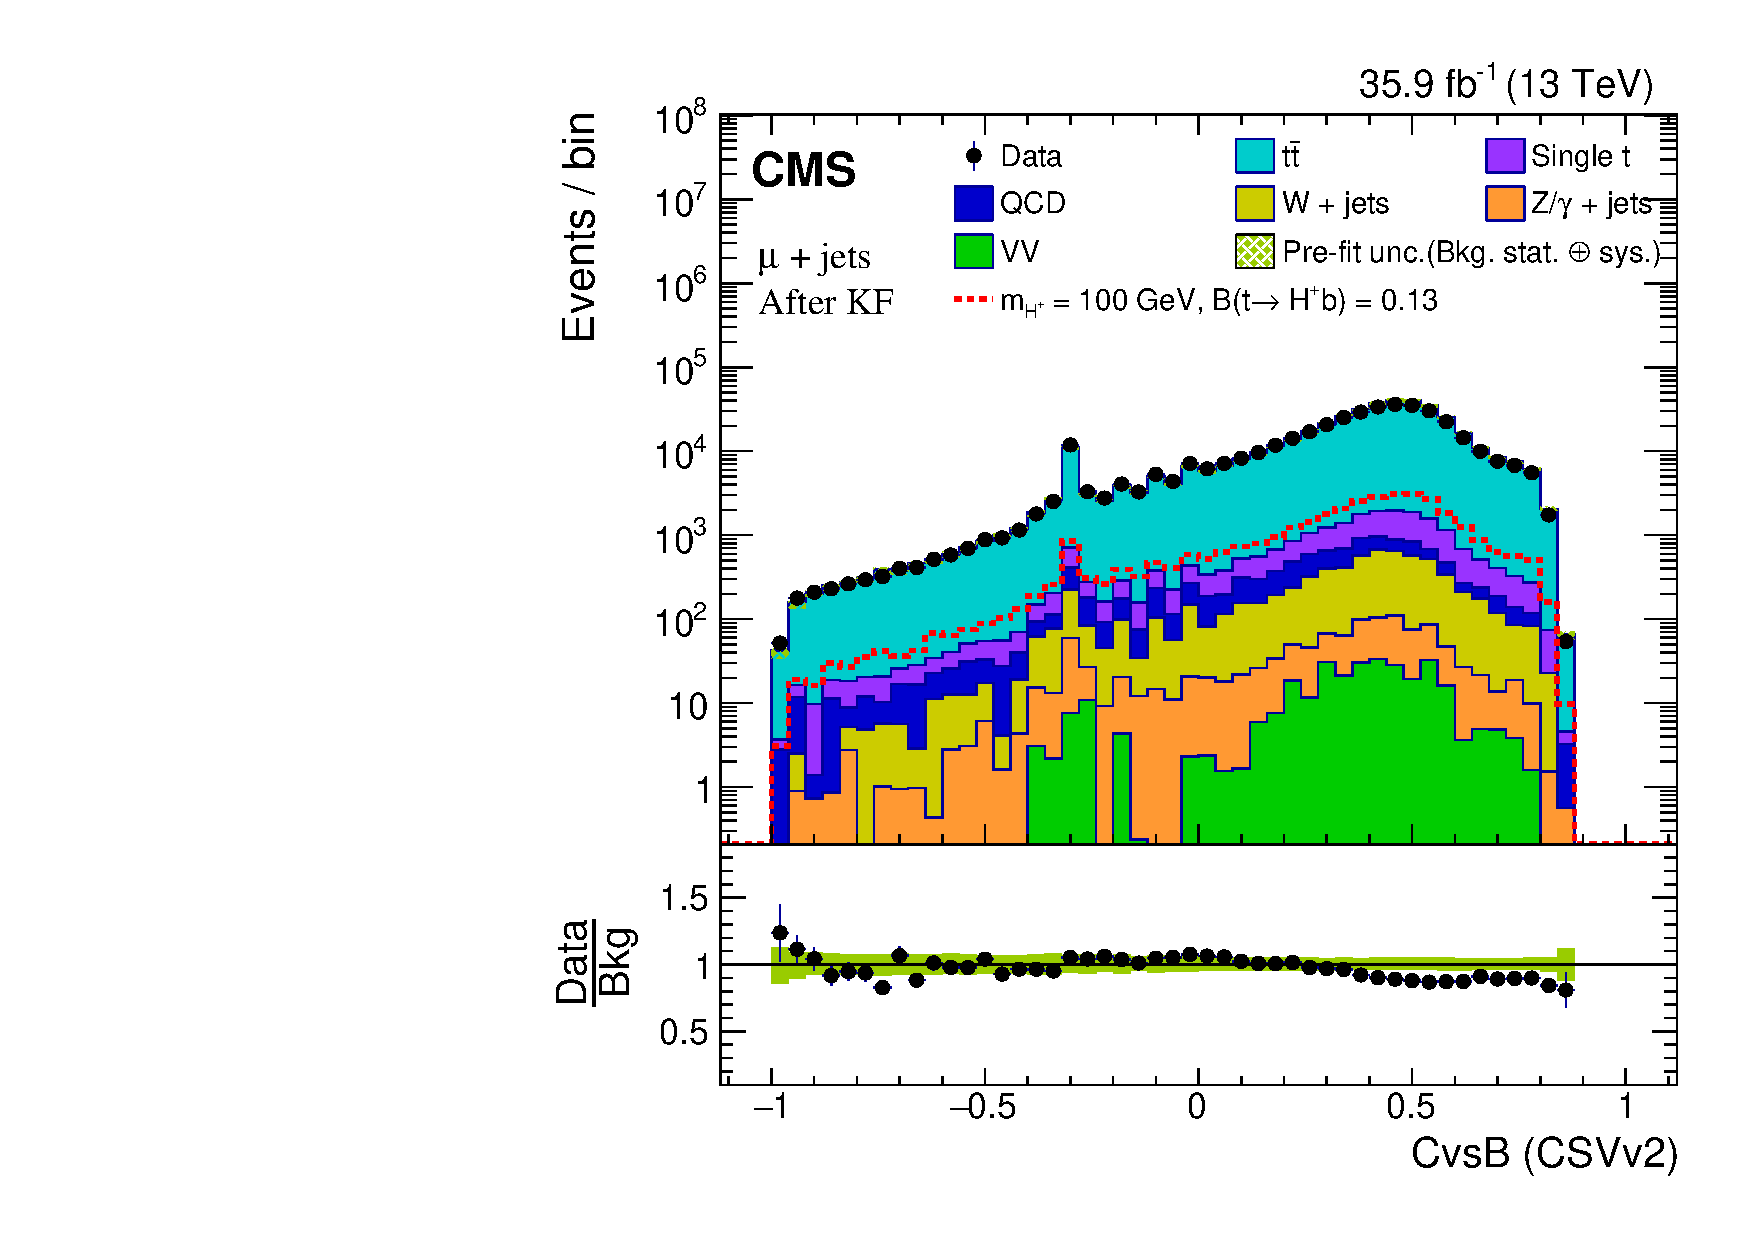
\includegraphics[width=0.50\linewidth]{Image/Muon/KinFit/pfCCvsB_muKinFit.pdf}}
\subfigure[charm vs. b-jet discriminator ]{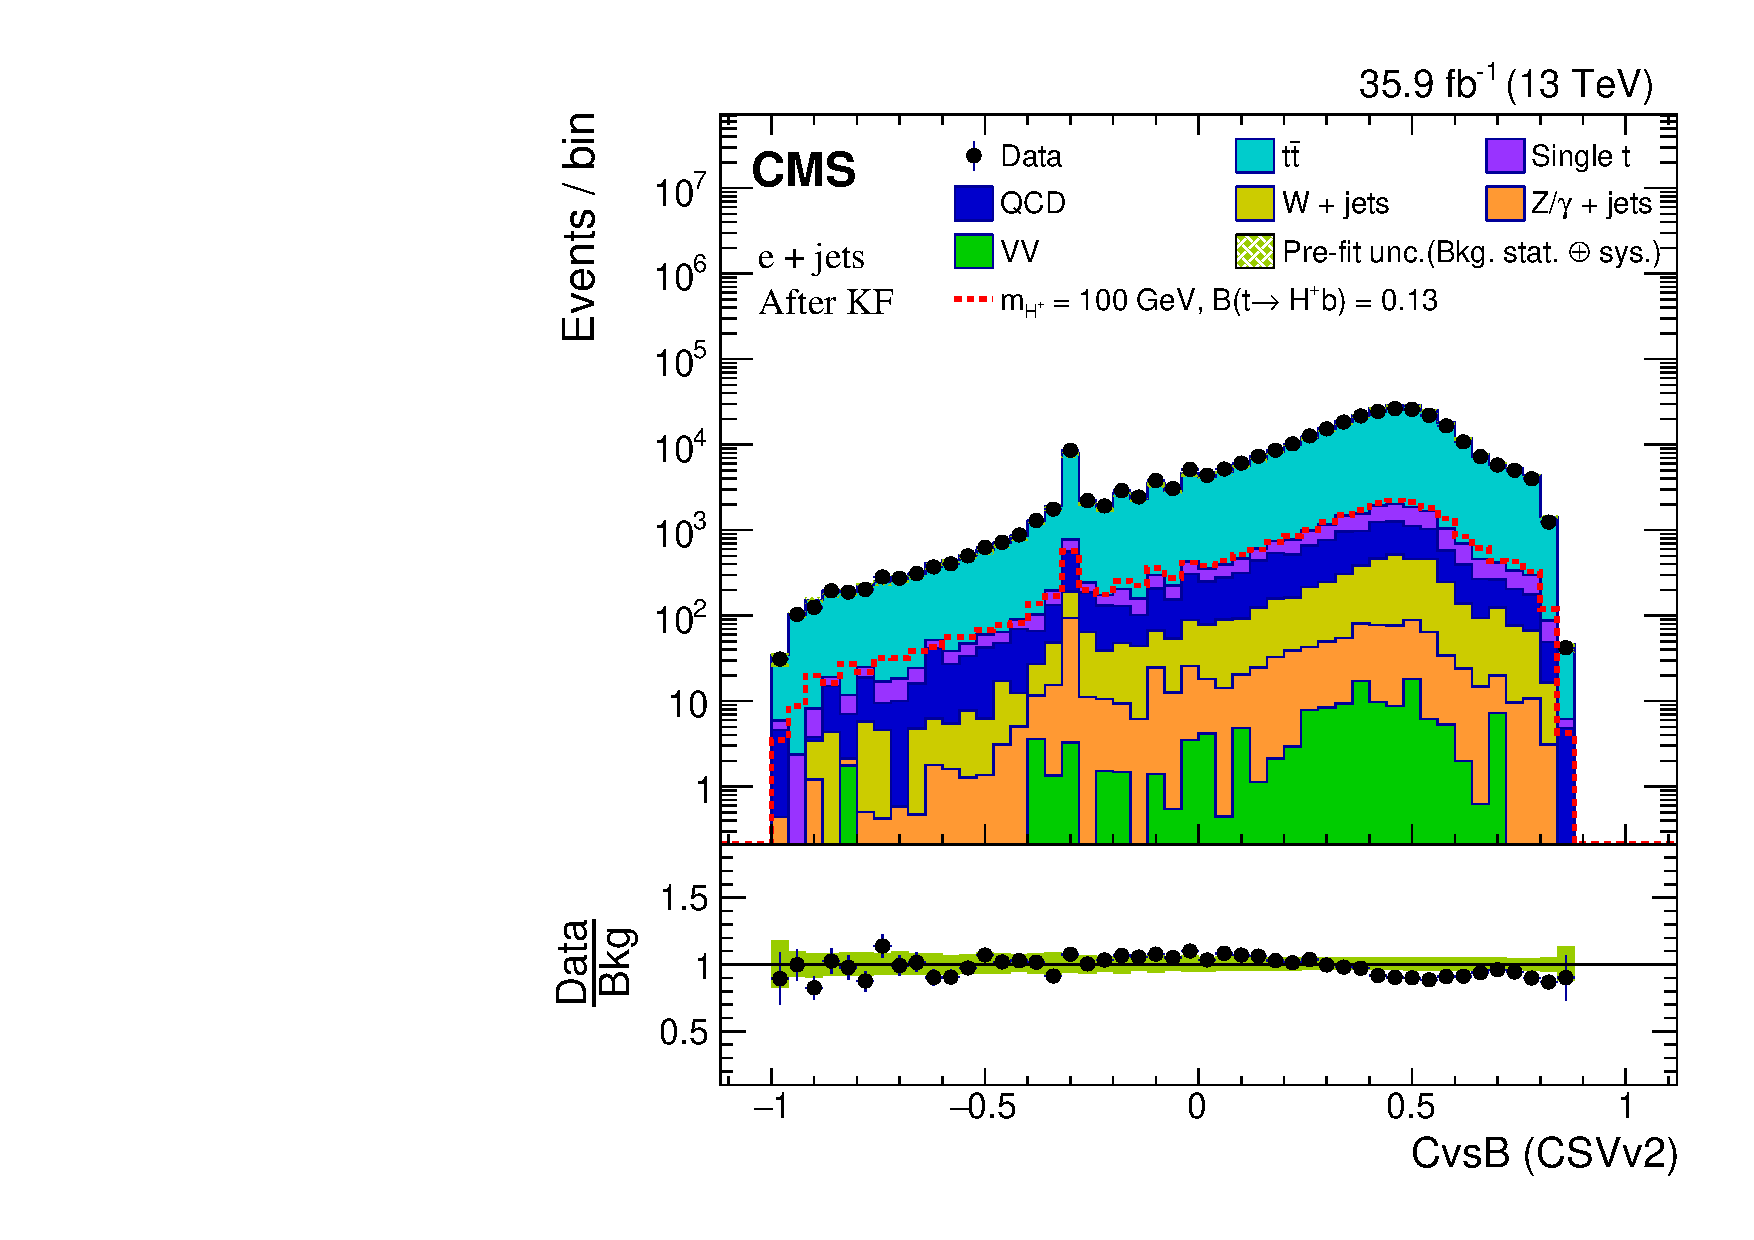
\includegraphics[width=0.50\linewidth]{Image/Electron/KinFit/pfCCvsB_eleKinFit.pdf}}
\vfil
\subfigure[charm vs. light jet discriminator ]{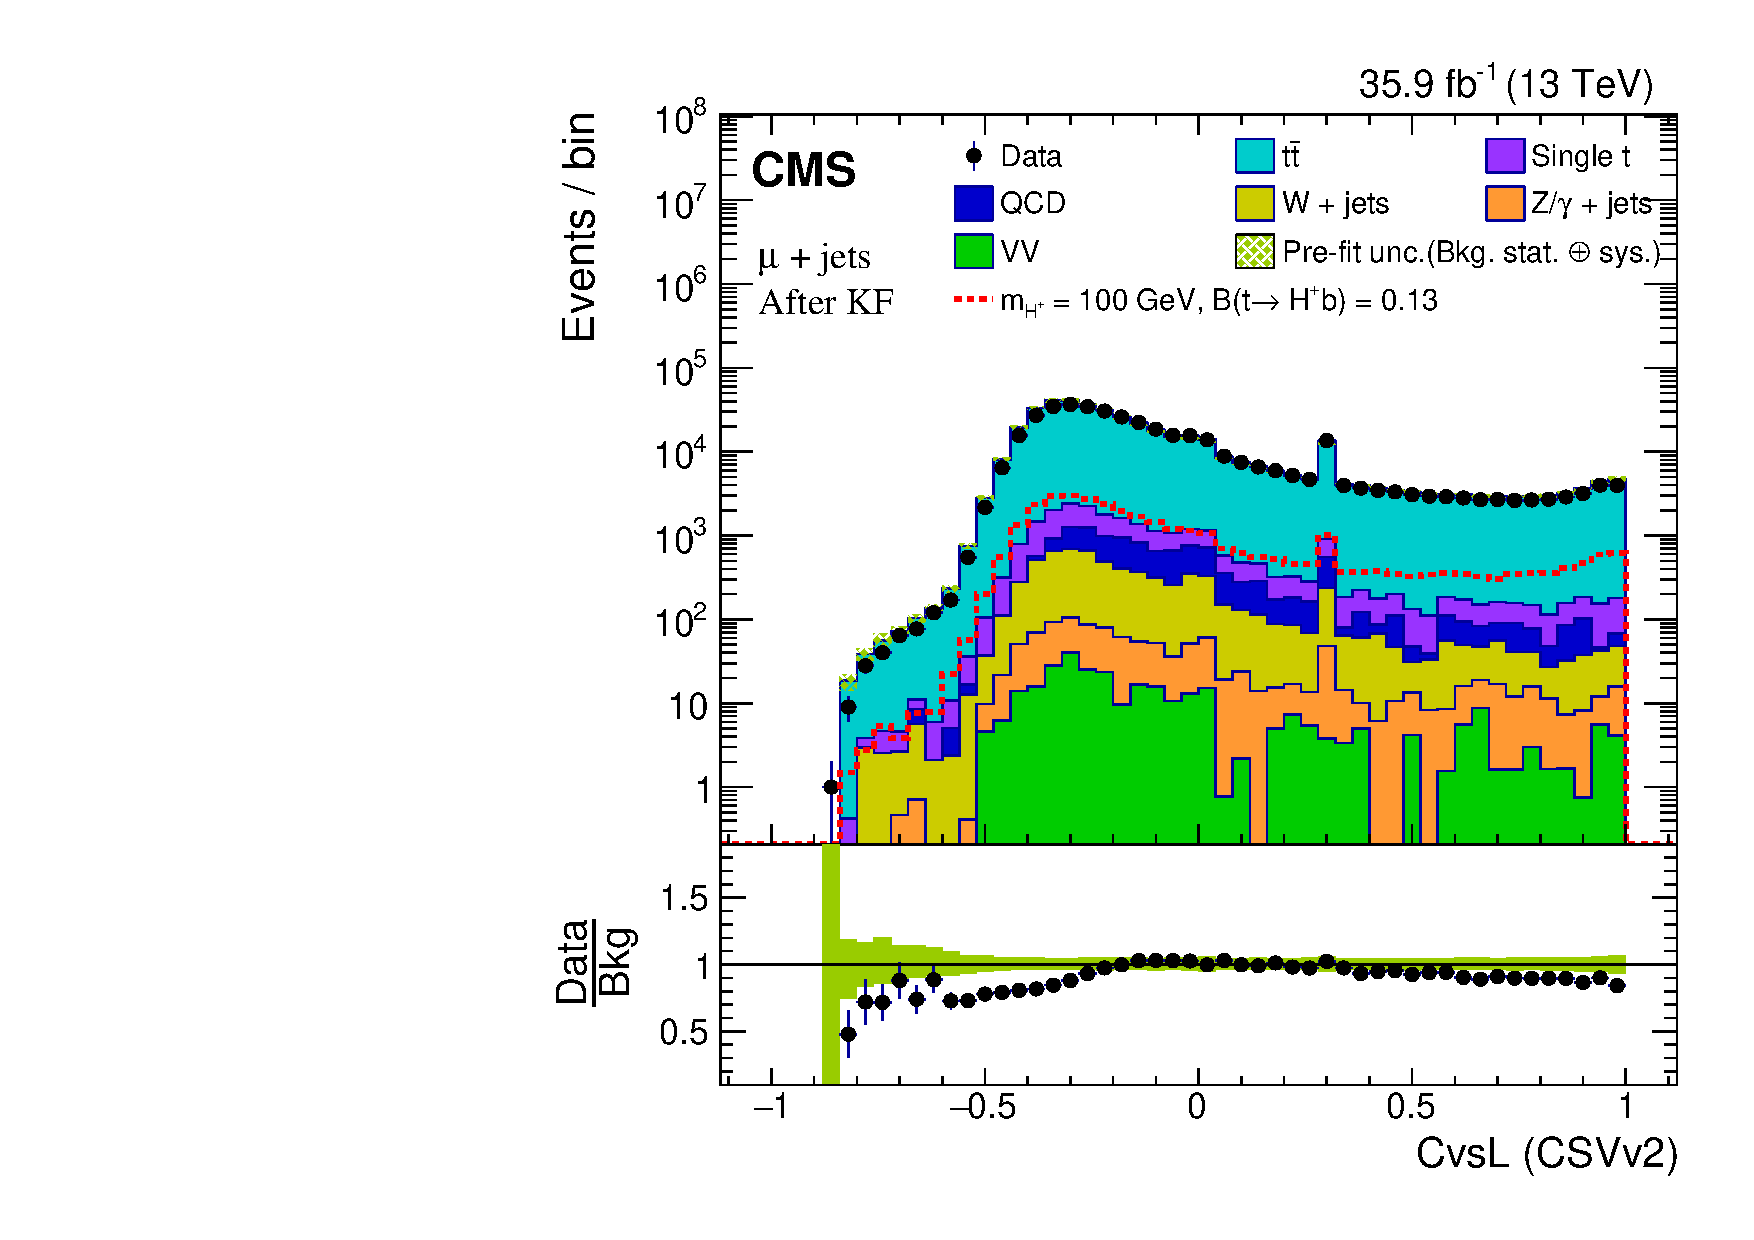
\includegraphics[width=0.50\linewidth]{Image/Muon/KinFit/pfCCvsL_muKinFit.pdf}}
\subfigure[charm vs. light jet discriminator ]{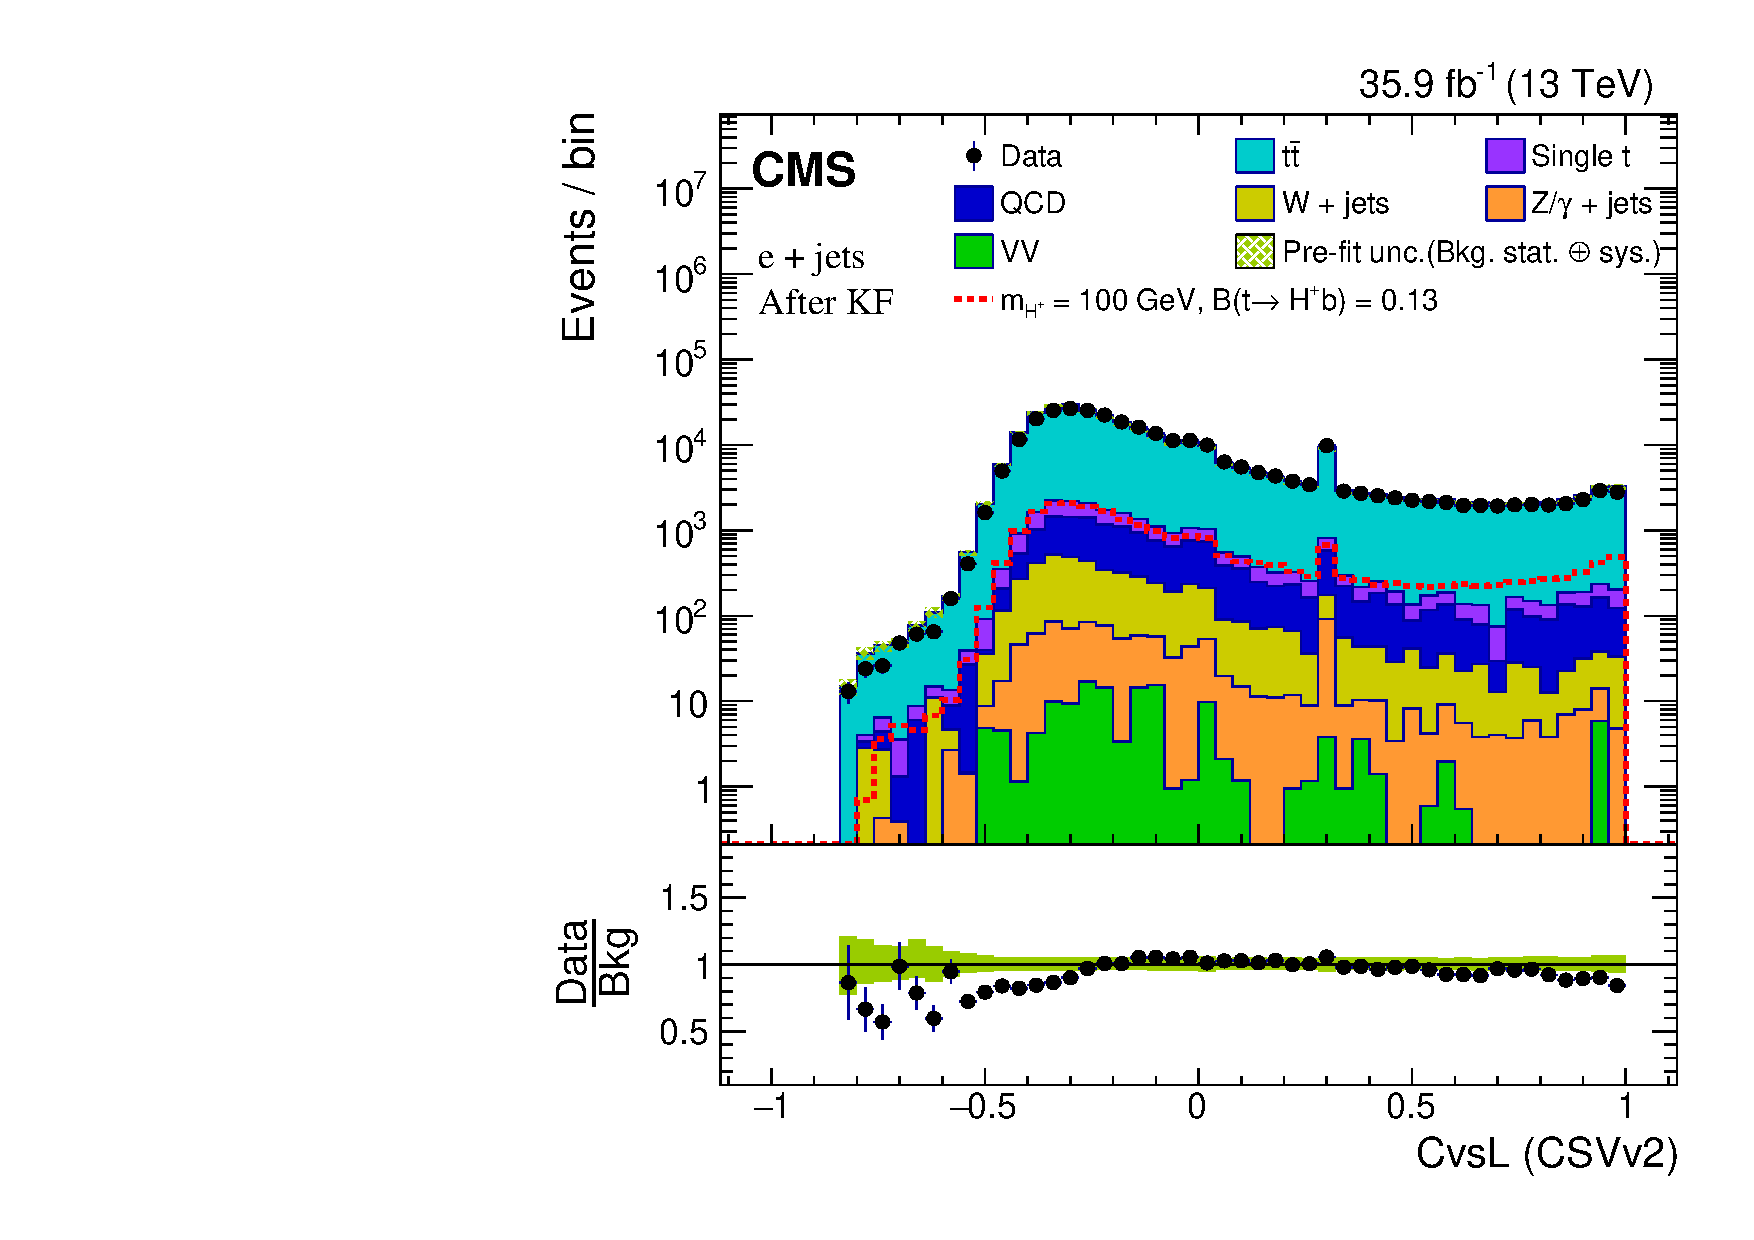
\includegraphics[width=0.50\linewidth]{Image/Electron/KinFit/pfCCvsL_eleKinFit.pdf}}
\caption{ The charm-discriminator distributions of two non-bjets after 
    kinematic fitting selection as described in Sec.~\ref{s:secEvtSel}, 
    obtained using the CSV method for the \mujets and \ejets channel.
    The jets with associated tracks not satisfying a set of selection criteria, 
    as listed in \cite{CMS-PAS-BTV-16-001}, are responsible for the spikes in 
    these distributions.} 
\label{fig:pfCCvsBL}
\end{figure}


